

% This is a semi-simple sample document.

\documentclass{article} % \documentclass{} is the first command in any LaTeX code.  It is used to define what kind of document you are creating such as an article or a book, and begins the document preamble

%\usepackage[spanish]{babel} % Para traducir palabras claves al español como "Figure" -> "Figura"

\usepackage{amsmath, amssymb} % \usepackage is a command that allows you to add functionality to your LaTeX code

\usepackage{mathtools} % using cases inside equations

\usepackage{graphicx} % image package

\usepackage{float} % Float specifiers are written in the square brackets whenever we use a float such as a figure or a table

\usepackage{subcaption} % more than one picture s in the same figure

\parskip 0.1in %paragraph distance

\usepackage[margin=0.984252in]{geometry} %margin

\usepackage[hidelinks]{hyperref} % Magic for index linking

\usepackage{chngcntr} % For figure number matching with section number
\counterwithin{figure}{section}

\usepackage{appendix} % Appendix

\pagestyle{headings} % Headings -> put the name of the section

%\pagestyle{myheadings} % Personalized headings
%\markright{whateveryouwant}

\title{Semi-Simple Sample Document} % Sets article title
\date{November 2021} % Sets article date

\author{
	\textbf{Ingeniería en Informática}\\
	Departamento de Tecnología y Administración\\
	\\~\\
	\textbf{Loiseau, Matías}\\
	mloiseau@undav.edu.ar
 	\\~\\
 	\textbf{Snow, Jon}\\
 	jsnow@winterfell.edu.ar
}

% The preamble ends with the command \begin{document}
\begin{document} % All begin commands must be paired with an end command somewhere

\begin{figure}
\centering
	
\includegraphics[width=0.2\textwidth]{images/undav-logo}
	%\caption{Mi Figure}
	\label{fig:undav-logo}
\end{figure}
\maketitle % creates title using information in preamble (title, author, date)

\thispagestyle{empty} % Ignore page number
\cleardoublepage

\cleardoublepage
\tableofcontents % general index
\cleardoublepage

\section{Forms to write text} % creates a section
Normal text

\textbf{Text in bold (ctrl + b)}

\textit{Text in italic (ctrl + i)}

Text with footnote\footnote{This is a footnote.}

This is a cite\cite{knn}.

\subsection{Enumerate and itemize information}

\begin{enumerate}
	\item Enumerate one
	\item Enumerate two
	\begin{enumerate}
		\item Sub-enumerate one
		\item Sub-enumerate two
	\end{enumerate}
\end{enumerate}

\begin{itemize}
	\item item one
	\item item two
	\begin{itemize}
		\item sub-item one
		\item sub-	item two
	\end{itemize}
\end{itemize}

\begin{enumerate}\addtocounter{enumi}{-1}
	  \item Start enumerate at 0
	  \item Enumerate one
\end{enumerate}

\section{Equations}

\subsection{Simple equations}

\begin{equation}
	E=mc^2
\end{equation}

\begin{equation}
	f(x) =
	\begin{cases*}
		1 & if x $>$ 0\\
 		0 & if x $\leqslant$ 0
 	 \end{cases*}
\end{equation}

\subsection{Complex equations}

\begin{equation}\label{eq:layers}
	\vec{h_1}^{\,} = f(\vec{x}^{\,}.W_1)
\end{equation}
	$$\vec{h_2}^{\,} = f(\vec{h_1}^{\,}.W_2)$$
	$$\vec{h_3}^{\,} = f(\vec{h_2}^{\,}.W_3)$$
	$$\vec{y}^{\,} = f(\vec{h_3}^{\,}.W_4)$$

\begin{equation}\label{eq:mse}
	MSE=\frac{1}{n}\sum_{i=1}^{n}(y_{i}-\hat{y}_{i})^2
\end{equation}

$$
\begin{pmatrix} a_0 & a_1\\ a_2 & a_3 \end{pmatrix}
\odot
\begin{pmatrix} b_0 & b_1\\ b_2 & b_3 \end{pmatrix}
=
\begin{pmatrix} a_0.b_0 & a_1.b_1\\ a_2.b_2 & a_3.b_3 \end{pmatrix}
$$

$$\frac{dL}{db_k}=\frac{dL}{dy_k}\frac{dy_k}{db_k}=\frac{dL}{dy_k}\frac{dy_k}{dz_k}\frac{dz_k}{db_k}=l'_{k+1}\odot f'_k\frac{d(W_kx_k+b_k)}{db_k}$$

\subsubsection{Matrix}

\begin{equation}
IoU(A,B)=\frac{|A \cap B|}{|A \cup B|}=\frac{|A \cap B|}{|A| + |B| - |A \cap B|}
\end{equation}

\cleardoublepage

\section{Figures} % creates a section

\begin{figure}[H]
	\centering
	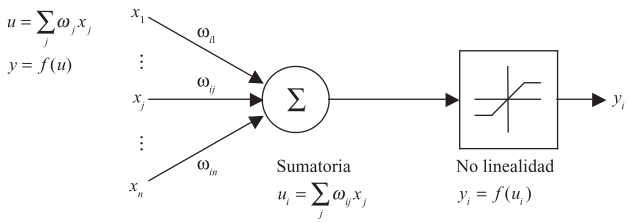
\includegraphics[width=0.8\textwidth]{images/perceptron-graph}
	\caption{Perceptron diagram.}
	\label{fig:perceptron-graph}
\end{figure}

This is a reference for the image (figure \ref{fig:perceptron-graph}) above.

\begin{figure}[H]
	\centering
	\begin{subfigure}{2in}
		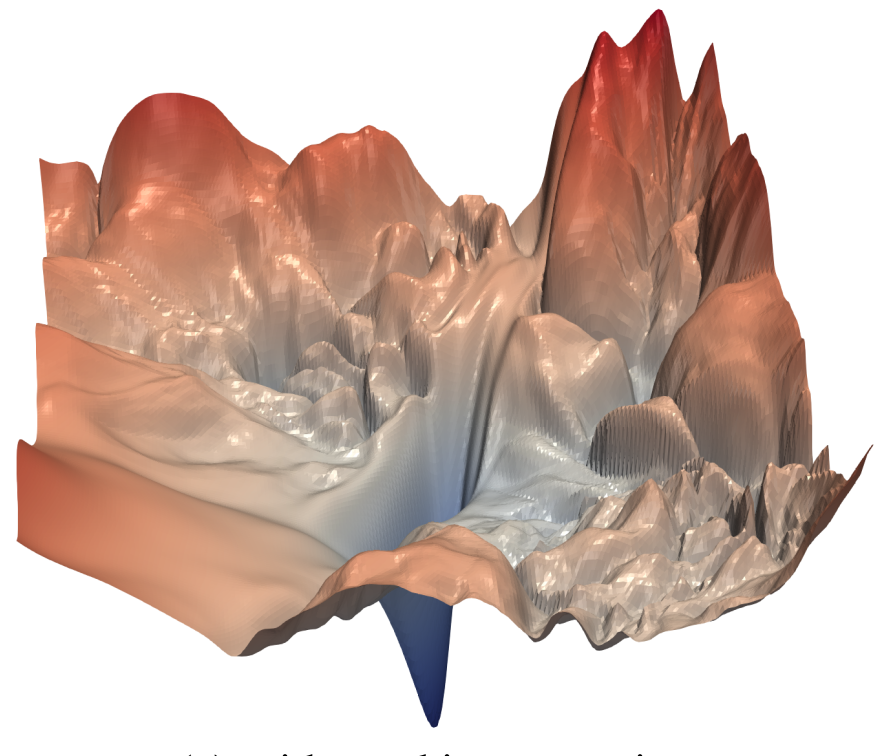
\includegraphics[width=1\textwidth]{images/mse-visu-1}
		\caption{Figure one.}
		\label{fig:mse-visu-1}
	\end{subfigure}	
	\begin{subfigure}{2in}
		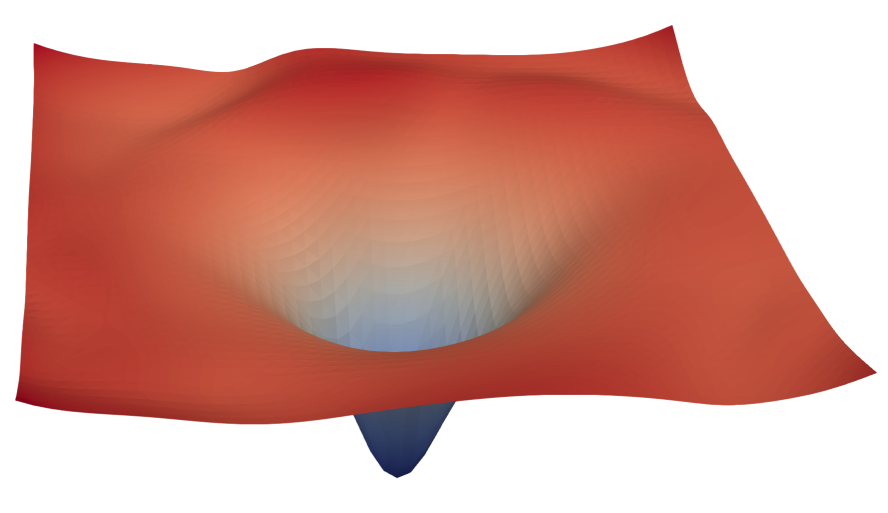
\includegraphics[width=1\textwidth]{images/mse-visu-2}
		\caption{Figure two.}
		\label{fig:mse-visu-2}
	\end{subfigure}
	\caption{Both figures.}
\label{fig:mse-visu-12}
\end{figure}

\section{Tables}

\begin{table}[H]
	\centering
		\begin{tabular}{||l | c ||}
			\hline
			\hline
			Data 1 & 185\\
			\hline
			Data 222 & 37\\
			\hline
			Data 333333 & 12\\
			\hline
			Data 4444444444 & 12\\
			\hline
			Data 555 & 13\\
			\hline
			\hline
		\end{tabular}
		\caption{Table X.}
	\label{tab:table-x}
\end{table}

\begin{table}[H]
	\centering
		\begin{tabular}{||l || c | c | c | c | c ||}
			\hline
			\hline
			& \multicolumn{3}{c|}{Number of people} & \multicolumn{2}{c||}{Difference between}\\
			\hline
			Module & 0 & 1 & 2 & 1 y 0 & 2 y 0\\
			\hline			
			\hline
			1 & 21.07 & 21.19 & 21.33 & 0.12 & 0.26\\
			\hline
			2 & 22.25 & 22.35 & 22.39 & 0.1 & 0.14\\
			\hline
			3 & 18.11 & 18.19 & 18.61 & 0.07 & 0.5\\
			\hline
			4 & 18.3 & 18.44 & 18.87 & 0.15 & 0.57\\
			\hline
			6 & 18.21 & 18.43 & 19.45 & 0.21 & 1.24\\
			\hline
			\hline
		\end{tabular}
		\caption{Table Y.}
	\label{tab:table-y}
\end{table}


\cleardoublepage

\appendix
\clearpage
\addappheadtotoc
\appendixpage

\section{First Appendix}\label{app:one}

This is an appendix

\cleardoublepage

\section{Second Appendix}\label{app:two}

Text

\cleardoublepage

\begin{thebibliography}{9}
\addcontentsline{toc}{section}{Bibliography} % This is for the bibliography appears in the index

\bibitem{iot}
Iván Federico Kwist, Matías Loiseau, David Exequiel Contreras, Federico Gabriel D’Angiolo,  Roberto Osvaldo Mayer. (2019). \textit{Monitorización de un Datacenter mediante Protocolos de IoT}. Congreso Nacional de Ingeniería Informática – Sistemas de Información.

\bibitem{regresion-lineal}
Federico Gabriel D’Angiolo, Iván Federico Kwist, Matías Loiseau, David Exequiel Contreras, Fernando Asteasuain. (2019). \textit{Algoritmos de Regresión Lineal aplicados al mantenimiento de un Datacenter}. Congreso Argentino de Ciencias de la Computación.

\bibitem{knn}
Federico Gabriel D’Angiolo, Iván Federico Kwist, Matías Loiseau , David Exequiel Contreras, Gregorio Oscar Glas. (2019). \textit{Algoritmo de KNN aplicado al mantenimiento de un Datacenter}. Congreso Nacional de Ingeniería Informática – Sistemas de Información.

\bibitem{deep-learning-nature}
LeCun, Y., Bengio, Y., \& Hinton, G. (2015). \textit{Deep learning}. nature, 521(7553), 436-444.

\bibitem{object-detection-review}
Zhao, Z. Q., Zheng, P., Xu, S. T., \& Wu, X. (2019). \textit{Object detection with deep learning: A review}. IEEE transactions on neural networks and learning systems, 30(11), 3212-3232.

\end{thebibliography}


\end{document} % This is the end of the document
